\documentclass[journal,transmag]{IEEEtran}

\usepackage{url}
\usepackage{graphicx}
\usepackage{pbox}
\usepackage{caption}

\hyphenation{op-tical net-works semi-conduc-tor}
\newcommand\MYhyperrefoptions{bookmarks=true,bookmarksnumbered=true,
	pdfpagemode={UseOutlines},plainpages=false,pdfpagelabels=true,
	colorlinks=true,linkcolor={black},citecolor={black},urlcolor={black},
	pdftitle={Bare Demo of IEEEtran.cls for Computer Society Journals},%<!CHANGE!
	pdfsubject={Typesetting},%<!CHANGE!
	pdfauthor={Michael D. Shell},%<!CHANGE!
	pdfkeywords={Computer Society, IEEEtran, journal, LaTeX, paper, template}}
\captionsetup{skip=10pt}

\begin{document}
	\title{Does Popularity Influence the Academy Awards?}
	\author{
		\IEEEauthorblockN{
			Fojan Babaali,
			Maryam Honari Jahromi,
			Omar Elazhary,
			Ali Mashreghi
		}
		\IEEEauthorblockA{
			University of Victoria, Victoria, Canada
		}
	}
	\IEEEtitleabstractindextext{
		\begin{abstract}
			In this project we are going to whether a movie's social profile data will be adequate to predict if that movie would get nominated or win an academy award. Our main data is the Kaggle IMDB movies dataset. We have added supplementary data about the history of Oscars' winners/nominees. We use the information after the movie was released since social media information -which is an important part of our features- only becomes stable a few months after release. We also intend to find the suitable algorithm to classify movies properly. Among the candidate algorithms are Naive bayes classifiers and linear regressors. We will also attempt to define a criteria by which movies are chosen.
		\end{abstract}
		\begin{IEEEkeywords}
			Oscars, Movies, Prediction, Classification, Machine Learning, Data Mining
		\end{IEEEkeywords}
	}
	\maketitle
	\IEEEdisplaynontitleabstractindextext
	\IEEEpeerreviewmaketitle
	
	\begin{enumerate}[Highlights]
\item In section \textit{Features Used in Prediction}, we have explicitly mentioned the features that we use for prediction.

\item In the whole process of feature selection we only consider training data.

\item After the mid-term report we tried AdaBoost and Neural Networks on our data.

\item We applied a rather new technique based on modulo to generate test/train set.
\end{enumerate}
	
	\section{Introduction}
	The Academy Awards, or "Oscars", is an annual awards ceremony to recognize excellence in cinematic achievements of a previous year's movies. These awards have been presented from 1929 and are known to mark distinguished performance in different categories which can bring fanfare.   
	
	One of the most controversial Oscar awards is the Best picture.
	Thirty-three of the films on the American Film Institute’s 100 Greatest Films were Academy Award Best Picture Winners.
	Seventy-five of the films were Academy Award Best Picture Nominees\cite{maryamref20}.
	This project attempts to examine if a highly popular movie is more likely to be nominated for or win an award.  We have implemented a number of classifiers to predict whether a movie will be nominated or win an award. The important questions that we intend to answer in this project are:	
	\begin{enumerate}
		\item Is a movie going to be nominated for Best Picture Award?
		\item Is a movie going to win Best Picture Award?
		\item How many academy awards overall a movie is going to win?
		\item Is social media data adequate enough to predict if a movie would be nominated for or win an award?
	\end{enumerate}	
	In this project, our main focus is to investigate how popularity and social media attention affects the oscars' results.
	\par
	This report is structured as follows: first an overview of the literature will be provided in the related work section. Afterwards, we will go over how we gathered and preprocessed our dataset. Next, we will discuss the methods used to classify and predict nominations and wins. Afterwards, the results will be illustrated and discussed along with what we hope to accomplish given more time.
	
	\section{Related Work}
	Some previous work has been done on predicting Academy Awards. A prediction was made for best picture, best actor, best actress and best director awards based on winning other awards, critics' ratings, bookie odds, genre and box office revenue\cite{ref1}.Since they were a business company we could not access their methods and data.
Another approach was done by sentiment analysis of IMDB discussion forums and weighing users based on their network positions. They were able to predict nine Oscar nominations correctly two months before announcement\cite{ref2}.We decided not to include text analysis into our project.
In one of the previous works, they collected the data by scraping Box Office Mojo and joining them with collected data from Open Movie Database (OMDB) API. For the sake of simplicity, they did data reduction and the final dataset had 516 movies of the original dataset which was gathered from Box Office Mojo with six major features including: Season, Rating, Genre, Total previous nominations, Metacritic Score, and Opening weekend gross. By applying the linear regression method, they tried to predict the number of Oscar nominations\cite{ref3}. We applied linear regression to our own dataset which has more movies and features.
Another approach which is related to our contribution is Academy Award Prediction. In this work, they tried to predict the 85th academy awards by focusing on aggregated rating, such as from audiences and critics on Rotten Tomatoes and IMDB. The data set was made up of a list of movies that have received at least a nomination in Best Film, Best Director, Best Actor or Actress groups of the Academy Awards. In this approach, they applied a couple of learning models. It seems for Best Actress results, SVM and Feature selected SVM; for Best Actor, multinomial naive bayes; for Best Director and for Best Picture, logistic regression and feature selected LR produced the best overall accuracy\cite{ref4}.
There is another study by David Kaplan which played with more smart features about film personnel and their Resume, genre and records in other award competition. Some of those features are:
\begin{description}
  \item[$\bullet$ ] If the film director won the DGA (Directors Guild of America) award
  \item[$\bullet$ ] Number of Best Actor Awards that the cast of film has previously won
  \item[$\bullet$] Number of Best Director awards for which the director of film has been nominated
\end{description}
It also showed the probability of winning Best Picture Award based on some hypothetical films with seven different sets of values. E.g. If chance of winning for film A is 8.8\% and its director wins the DGA Award, the chance increases to 96.7\%. He used a couple of logistic regression models with a combination of different features. The best result was 97.7\% accuracy on predicting whether a film wins Best picture award or not\cite{ref5}.
Although there are many approaches that have been done in award-prediction, only a few of them have paid attention to Oscar Prediction. In this project, we are going to present our contribution by using a dataset and learning methods in order to predict oscars winners and nominations, based on which we will assess whether or not social media data is adequate for this task or not.
	
	
	\section{Data Gathering and Description}
As mentioned previously, our main dataset was a collection roughly 5000 movies from Kaggle created by \emph{Mr. Chuan Sun} \cite{refCreator}. However, since we needed some features to be able to predict Oscar nominees and winners we started gathering historical data. To do this, we wrote a crawler in Java which went through the search results of the official Oscars' website (\url{http://www.oscars.org}) and collected all necessary information on winners and nominees from as early as 1916. Our crawler does that simply by parsing the html pages returned as search result. It also gathers the names of people who won a specific award.\\
Important features that we added were whether each movie in the dataset was nominated for each category or not. Also, we added features that tell us whether the movie has won a specific award or not (Figure \ref{fig4}). Based on this, we added a column which specifies the number of awards won by a movie. However, when we want to predict if a movie is going to be nominated for Best Picture we ignore all other features regarding nomination. The reason is that this kind of prediction is supposed to be used on the time before nominees' names are released. Similarly, when we aim at predicting if a movie is going to win an award or not, we ignore features regarding winning other awards. The reason again is that this classifier is supposed to be used before Oscars' ceremony. The same goes for predicting number of awards for which we ignore the columns that say whether the movie has won an award.\\
\textbf{Note:} Though we never use \emph{Award Winning Features}, we still include them in the dataset to facilitate the process of analyzing our results. For example, when we want to see the information on some movie that is always classified wrong we may use these information to get a better understanding of our data.\\

\subsection{Missing Movies}
The dataset that we downloaded from Kaggle has mostly social media and popularity features (e.g. movie facebook likes, imdb score). Our main goal in this stage is to predict Oscar winners/nominees. With that in mind, there were near 250 movies which were nominated for the Best Picture Award over the past century but were absent in our dataset; hence, we collected the titles of these movies using our Java crawler and also repeated the work of Chuan Sun (creator of the dataset) to add the missing 250 movies. To do this we used the information provided on this blog \cite{refCreator}. \\
An important point is that the way that IMDB links are retrieved in Chuan Sun's codes is a little bit problematic. It first searches for the title of the movie in IMDB using IMDB's search API, and after that uses the first link in the result as the link for the movie. However, this does not always work fine since sometimes the order of the results is not as desired. So, we refined this part of code to consider the link whose related title matches the title that we have. This way we managed to reduce the number of mistakes.

\paragraph*{Movies from 2016} We first retrieved the titles of 100 good 2016 movies from  \url{rottentomatoes.com} and used Chuan Sun's code to collect social and IMDB information on these movies. We used this dataset to predict potential nominees for the upcoming Oscar ceremony in 2017. 

\begin{figure}

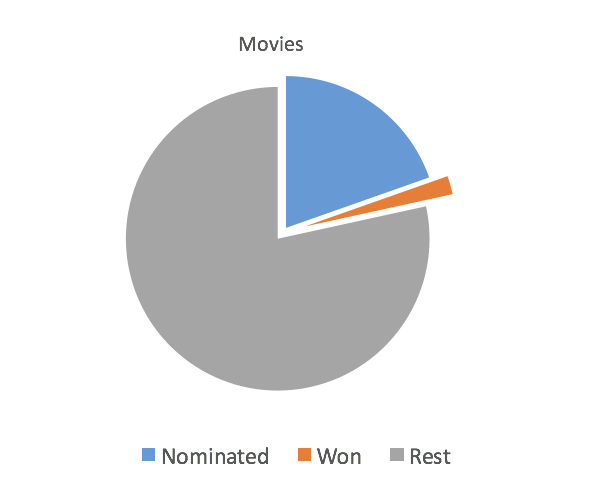
\includegraphics[scale=.45]{fig1.png}
 \caption{Distribution of movies according to best picture nominated/winner statistics.}
\label{fig4}
\end{figure}


\begin{figure}

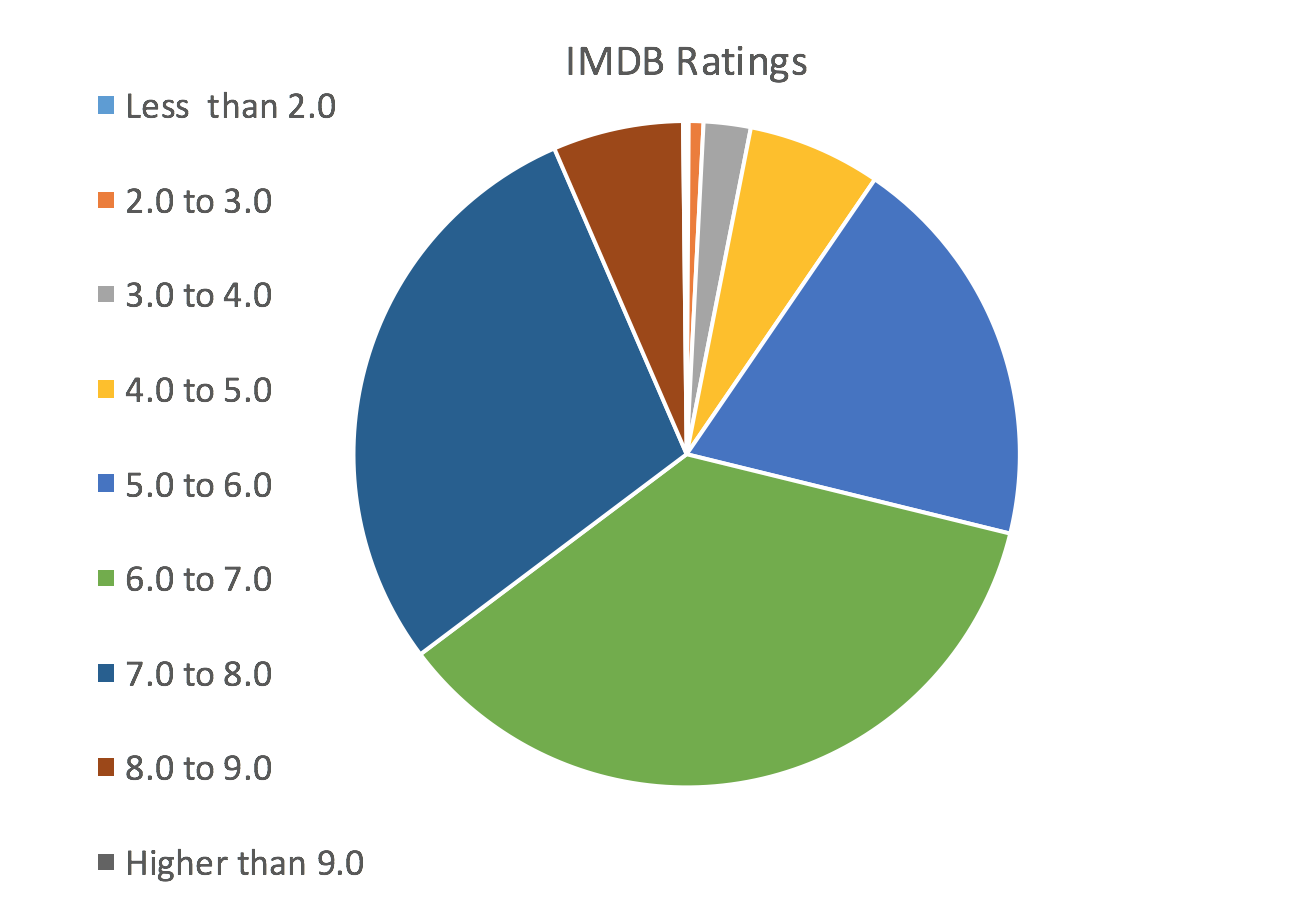
\includegraphics[scale=.5]{fig22.png}
 \caption{Number of movies based on IMDB rating.}
\label{fig1}
\end{figure}

\begin{figure}

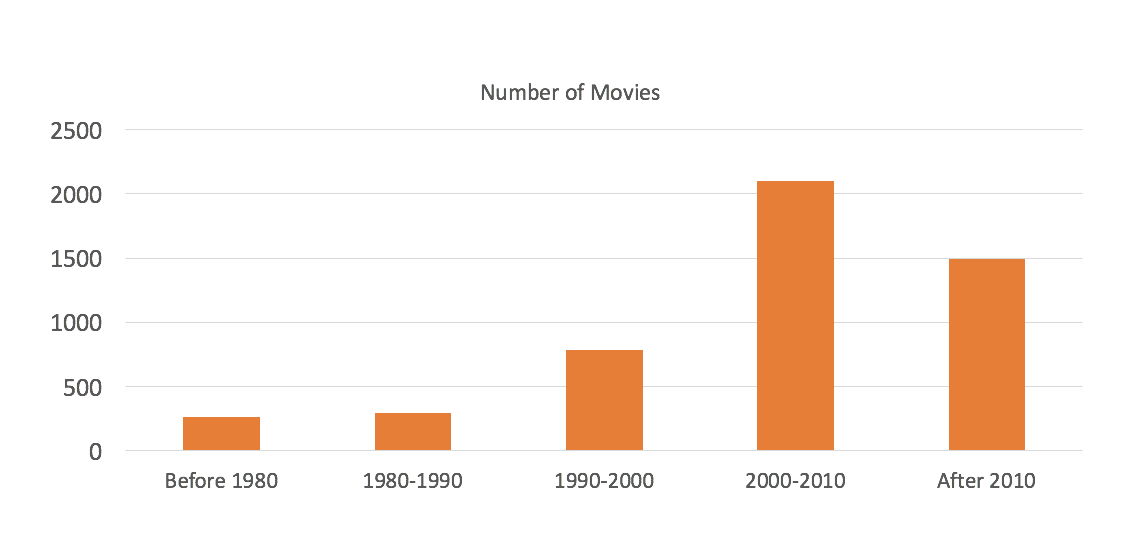
\includegraphics[scale=.22]{fig2.png}
 \caption{Number of movies based on year.}
\label{fig2}
\end{figure}

\begin{figure}

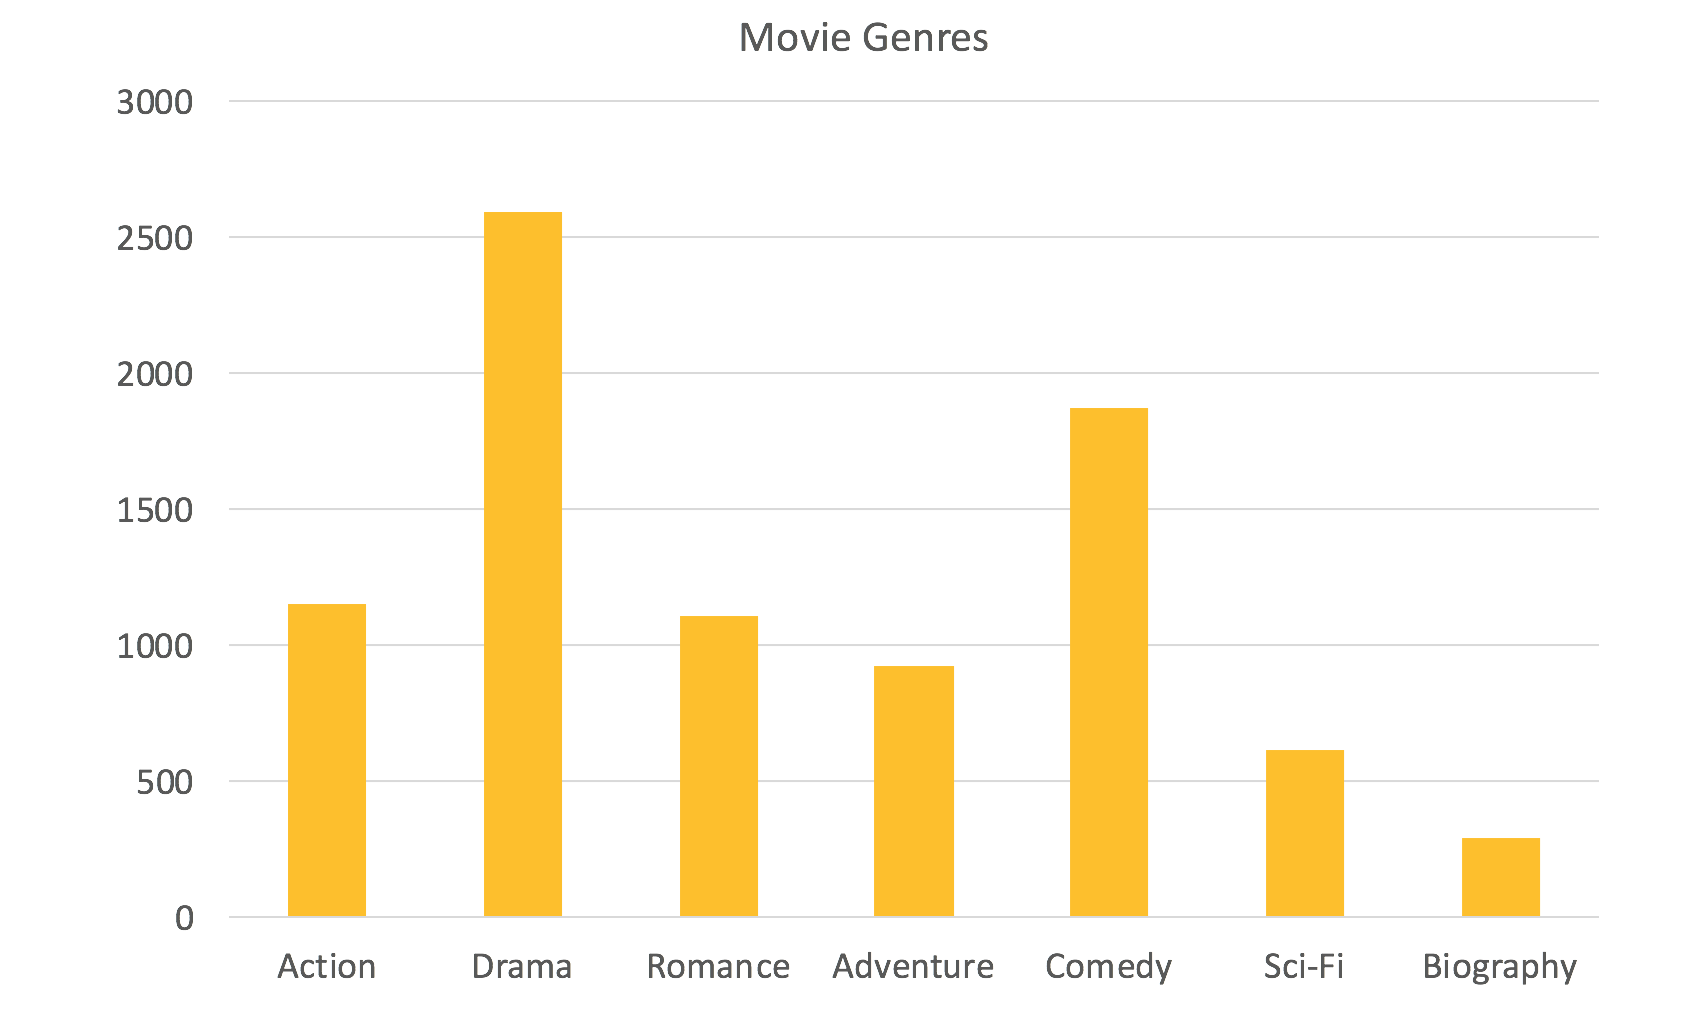
\includegraphics[scale=.30]{fig3.png}
 \caption{Number of movies based on genres.}
\label{fig3}
\end{figure}

\subsection{Some Data Statistics}
We have nearly 5000 movie titles in our dataset. Some statistics about these movies are as follows:

\begin{enumerate}
\item{\textbf{IMDB score:}} IMDB score is an important feature in our dataset. Figure \ref{fig1} shows a pie diagram on distribution of movies based on rating.

\item{\textbf{Title year:}} Naturally, in recent years the number of movies have grown rapidly and our dataset reflects this growth, as well. Overall, as illustrated in Figure \ref{fig2}, we have 261 movies earlier than 1980, 291 movies in 1980-1990, 786 movies in 1990-2000, 2100 movies from 2000 to 2010, and finally 1497 movies from 2010 to present time.

\item{\textbf{Director:}} There are 2399 directors involved in these movies. There are 36 directors who have at least starred in 10 movies each. Top directors by the number of movies they have in our dataset are: Woody Allen with 22 titles, Clint Eastwood with 20, Martin Scorsese with 20, Ridley Scott with 17, and Steven Soderbergh, Spike Lee and Tim Burton all with 16 movies. Also a total of 2363 directors have less than 10 and 1537 directors who have only one movie in our dataset.

\item{\textbf{Actor/Actress:}} There are 6258 actors/actresses involved in all these movies. There are 222 that have acted in at least 10 movies, and 6036 who have acted in less than 10 movies. Top actors/actresses by the number of movies are: Robert De Niro with 54 movies, Morgan Freeman with 47 movies, Johnny Depp with 41 movies, Bruce Willis with 40 movies, Matt Damon with 38 movies, and Steve Buscemi with 37 movies. Also 3901 actors/actress are present in our dataset who have been involved in one movie only.

\item{\textbf{Genres and plots:}} Among the most frequent genres are Action, Drama, Romance, Adventure, Comedy, Sci-Fi and Biography. The most frequent genre is obviously Drama. And after that Comedy, Action and Romance follow. Figure \ref{fig3} shows how many movies include each of these genres. Furthermore, plot keywords are another feature in our dataset. However, in order to be able to use them, we split keywords from genres and plots to different columns. Though this resulted in a huge matrix, we were able to get some important keywords such as \emph{racism} and \emph{suicidal thoughts} that help us in both classification and regression.

\item{\textbf{Social networks}} The only social network information that is present in this dataset are facebook likes of movies, directors, actors/actresses and cast members overall. The highest movie facebook likes belongs to Interstellar with 349000 likes, then Django Unchained with 199000 likes, Batman v Superman: Dawn of Justice with 197000 likes and Mad Max: Fury Road with 191000 likes. There are 749 movies that have less than 1000 likes on facebook.
\end{enumerate}

\subsection{Description of All Features}
\begin{figure}
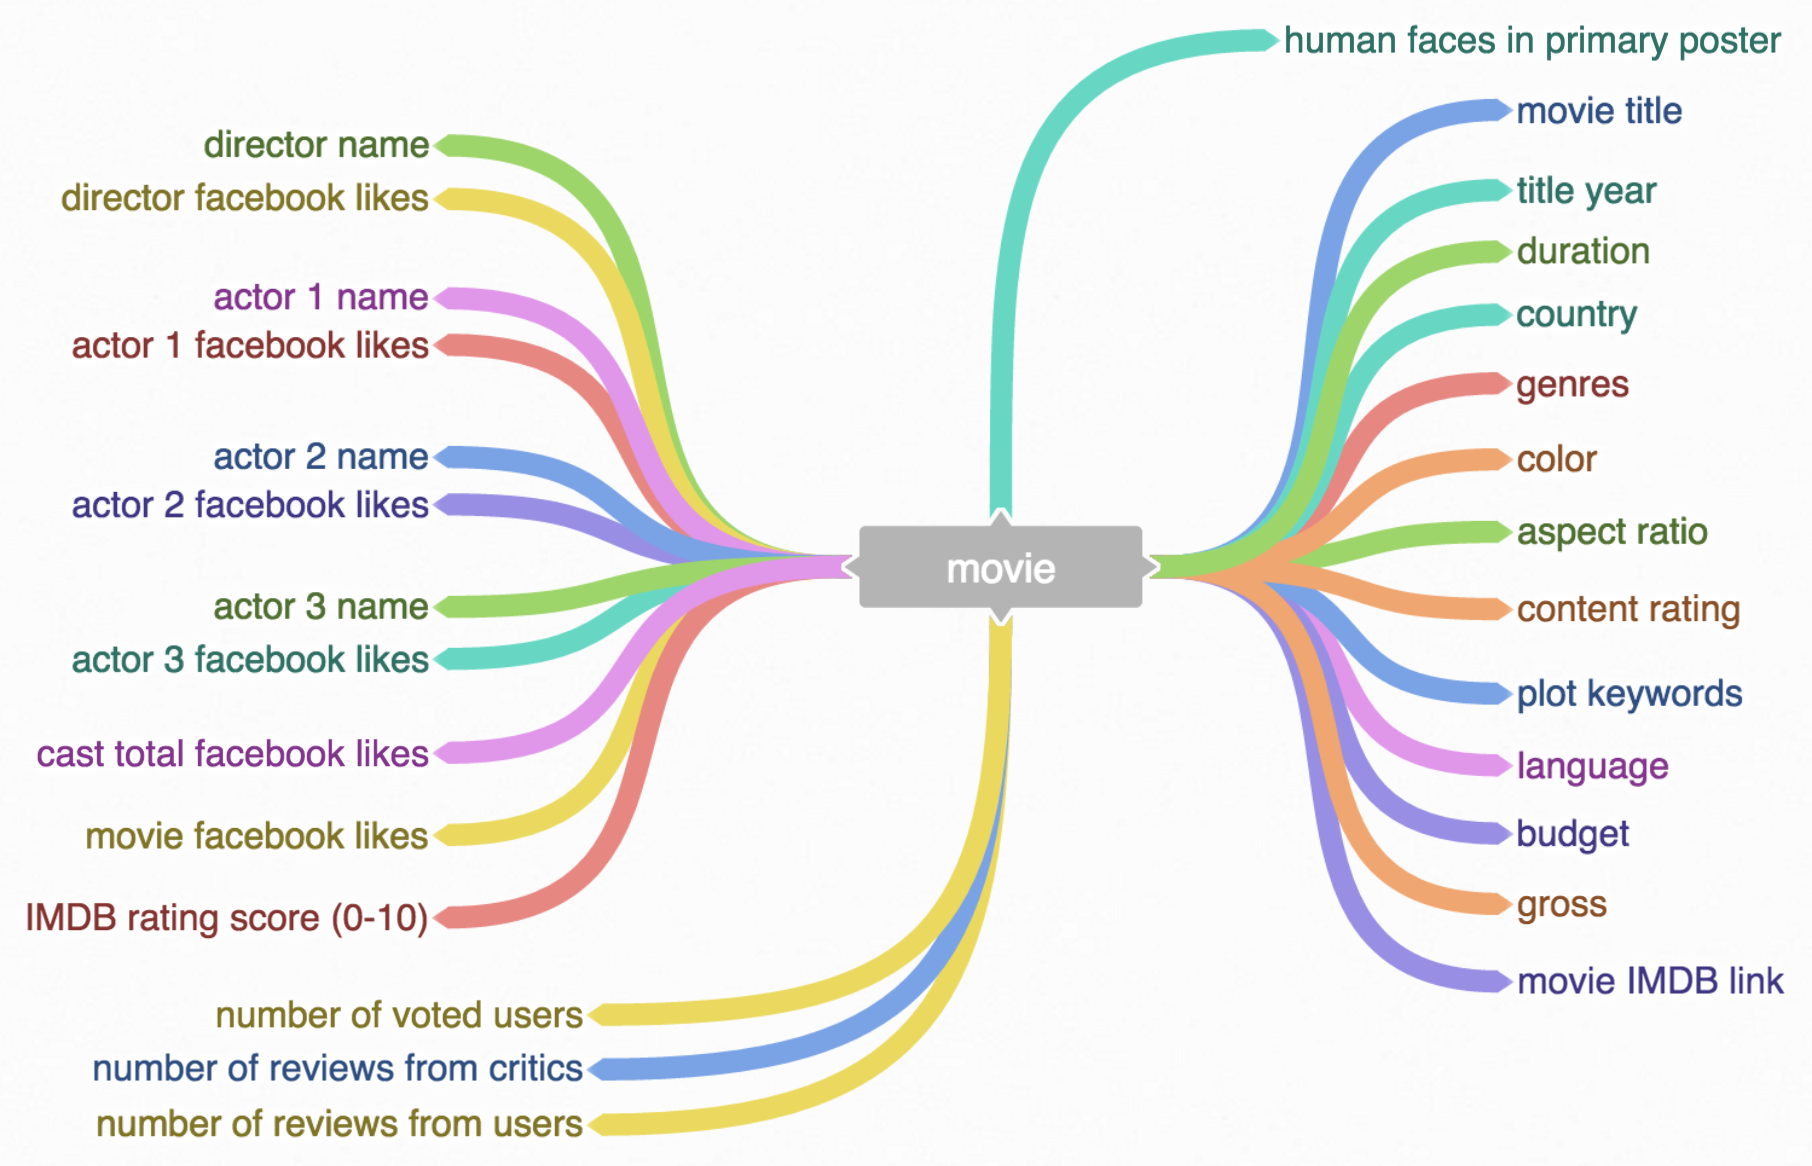
\includegraphics[scale=.22]{fig_feat.png}
 \caption{Features in our dataset}
\label{fig_feat}
\end{figure}

Now, we aim to describe each of the features present in our dataset. A simple diagram showing the name of all initial features of the Kaggle dataset downloaded from \cite{refCreator} can be found in Figure \ref{fig_feat}.

\begin{enumerate}
\item{\textbf{\textit{color:}}} Shows the color of the movie. Its value can be either \textit{Black/White} or \textit{Color}.

\item{\textbf{\textit{director name:}}} The name of the director as a string of characters.
\item{\textbf{\textit{director facebook likes:}}} Number of likes on director's facebook page.
\item{\textbf{\textit{actor X name:}}} X can be 1, 2 or 3. It is the name of the first, second or third most important actor/actress. 
\item{\textbf{\textit{actor X facebook likes:}}} The number of likes on the actor/actress's facebook page.
\item{\textbf{\textit{cast total facebook likes:}}} The overall number of facebook likes on pages of all cast and crew.
\item{\textbf{\textit{movie facebook likes:}}} Number of facebook likes of the movie. 
\item{\textbf{\textit{imdb score:}}} The rating of the movie on IMDB which is a number with one floating point between 0 and 10.
\item{\textbf{\textit{num voted users:}}} Number of users who rated the movie on IMDB.
\item{\textbf{\textit{num user for reviews:}}} Number of users who wrote a review for the movie on IMDB.
\item{\textbf{\textit{num critic for reviews:}}} Number of critics who wrote a review for the movie on IMDB.
\item{\textbf{\textit{facenumber in poster:}}} Number of human faces on the primary poster of the movie.
\item{\textbf{\textit{plot keywords:}}} Keywords in the movie plot separated by pipe ($|$) character. We split these features into \textit{keyword=} columns.
\item{\textbf{\textit{keyword=X:(Added by us)}}} X is a word or collection of words. This feature is binary; 1 if the keyword is found in \textit{plot keywords}, 0 otherwise.
\item{\textbf{\textit{genres:}}} Genres of the movie separated by pipe ($|$) character. We split these features into \textit{genre=} columns..
\item{\textbf{\textit{genre=X:(Added by us)}}} X is a genre of movie. This feature is binary; 1 if the keyword is found in \textit{genres} feature, 0 otherwise.
\item{\textbf{\textit{movie title:}}} The name of the movie as a string.
\item{\textbf{\textit{title year:}}} The year that the movie was released.
\item{\textbf{\textit{duration:}}} Duration of the movie in minutes.
\item{\textbf{\textit{country:}}} The country that produced the movie.
\item{\textbf{\textit{aspect ratio:}}} Aspect ratio of the movie, for example if the screen is 16:9, the ratio will be 1.78.
\item{\textbf{\textit{content rating:}}} Content rating of the movie, e.g. PG 13 which is not appropriate for children under 13.
\item{\textbf{\textit{language:}}} Language of the movie.
\item{\textbf{\textit{budget:}}} The budget of the movie.
\item{\textbf{\textit{gross:}}} Gross income of the movie.
\item{\textbf{\textit{movie imdb link:}}} The url of the movie on IMDB.
\item{\textbf{\textit{Nominated X: (Added by us)}}} A binary feature indicating whether a the movie has been nominated for award category X. For example, \textit{Nominated Art Direction}
\item{\textbf{\textit{Won X:(Added by us)}}} A binary feature indicating whether a the movie has won a specific award X. For example, \textit{Won Art Direction}
\item{\textbf{\textit{Num of Awards:(Added by us)}}} The number of all awards won by that movie. This is basically the sum of \textit{Won X} features for that movie.
\end{enumerate}

\textbf{Note:} The columns \textbf{Nominated Best Picture}, \textbf{Won Best Picture} and \textbf{Num of Awards} turn into our class labels to predict.

\subsection{Preprocessing and Refining the Dataset}
The first thing that we did for refining our data was to remove mistakes from the \textit{year} feature. In the original dataset in many cases the years extracted from IMDB are wrong. However, we knew that a lot of movies in our dataset have been nominated for at least one Academy Award. Therefore, using the results of our crawler we could retrieve the correct year of the movies and replace them in the dataset.\\

Then we moved on to preprocessing the data. Firstly, the data is loaded from the csv file. Since everything that is read by python from csv is essentially a string type, each value is checked for its convertibility to a numeric type, and then converted accordingly. Empty values represented by '' are converted to the standard numpy ``NaN" value. The result of this process is two typed 2D arrays, the first containing features as specified by the preprocessor formatted as $[$ \textit{$<$number-of-samples$>$, $<$number-of-features$>$} $]$, and the second contains class labels formatted as $[$ \textit{$<$number-of-labels$>$, $<$number-of-samples$>$} $] $.\\
The second step is essentially dealing with all empty/missing values from the earlier step. This is accomplished by using scikit-learn's ``Imputer" functionality. The ``Imputer" function is used on a per-feature basis (labels are assumed not to hold empty values). As a filling strategy, the \textit{most-frequent} mode is used. The reasoning behind this is quite simple. These are mostly categorical data, i.e. director names, actor names, and others. The mean, in this case, would make no sense. The median could be used, as it represents a single value, however, it does not accurately give a sense of how the data is distributed. Neither does the mode, for that matter, however, it is the most logical choice among the three. Ideally, the dataset would be complete, or need to be completed by hand in order to fill in the gaps. So, this could be considered a weakness.\\
The third step is converting all categorical data into numerical data capable of being processed by scikit-learn's methods. This is done using scikit-learn's ``LabelEncoder" functionality, which results in string values being mapped to numbers (usually their indices in an array). These are then substituted into the data. Another alternative was to pipe the result of the ``LabelEncoder" through a ``OneHotEncoder" to apply the binary technique discussed in class. This, however, would result in a larger matrix. And given the larger number of features that had been initially identified (roughly 8000), increasing the matrix size would be considered disadvantageous, and was abandoned in favor of just using the ``LabelEncoder".


\subsection{Feature Selection and Dimensionality Reduction}
Two of the features already given in the dataset consist of delimited genres and plot keywords. These were expanded into unique values per genre and unique values per keyword. Each additional feature would be encoded as a boolean flag, whereby if a movie is assigned a particular genre/keyword, its corresponding flag would be switched on (1), otherwise it would be switched off (0). This resulted in a large amount of extra features.\\
Due to the large amount of features and the large time consumed by processing them, a feature selection and dimensionality reduction strategy was considered. Pearson's correlation coefficient was calculated for each feature and each label. The feature-label combinations whose absolute correlation was greater than 0.1 (i.e. strength of the correlation, regardless of its nature) were the ones considered later for classification/regression. Variations based on team-member judgement on what would improve classification quality were later used. This is discussed later with each individual algorithm applied.\\
\textbf{Note:} As Dr. Fyshe pointed out, we were careful to select important features only using our training data, since including test data in feature correlation results in overfitting. \\

\subsection{Features Used in Prediction}
Basically, when we want to predict each of the class labels (i.e. Best Picture Nominee, Winner and Number of Awards) we use all the features whose correlation value the desired class label is above 0.1. (This selection of features is based only on the Training Data.) The reason for this threshold is that except for \textbf{\textit{Nominated X}} features most of our correlation values are below 0.2 and if we do consider a rather high threshold there will not be enough features for the classifier/regressor to use. Here is the list of features that we use for prediction. Note that we only mention some of the \textbf{\textit{keyword=X}} and \textbf{\textit{genre=}} features as there are quite a few. Also, we mention any feature whose correlation result with respect to \textit{at least} oen class label is above 0.1.\\
Original Features Used in Prediction:\\
\textit{\textbf{ color, duration,	gross,	num\_voted\_users, 	facenumber\_in\_poster,	num\_user\_for\_reviews,	country,	title\_year,	imdb\_score	, movie\_facebook\_likes}} \\

\noindent
Nominated X Features Used in Prediction:\\
\textit{\textbf{Leading Actor/Actress, Supporting	 Actor/Actress, Art Direction, Cinematography, Costume Design, Directing, Film Editing, Makeup,  Music Scoring, Music Song, Sound, Sound Editing, Visual Effects, Writing }}\\ 
(Notice that features such as Best Animated Movie are ignored)\\

\noindent
Some of the Used Genres and Plot Keywords:\\
\textit{\textbf{genre=Romance,	genre=Action,	genre=War,	genre=Thriller,	genre=Biography,	 genre=History,	genre=Drama, keyword=jazz age,	keyword=broadway play,	keyword=gallantry,	keyword=republic,	keyword=casablanca morocco,	keyword=visa,	keyword=boer war,	keyword=longshoreman	, keyword=rose, 	keyword=dangerous job,	keyword=coin toss}}

\subsection{A New Technique for Generating Test and Train Sets} \label{train_test_set}
There are a number of ways to generate test/train sets. However, not all of them seem reasonable. For example, generating test/train sets using randomness does not seem logical because the number of Best Picture nominees/winners is small compared to the number of movies in our dataset. So, if we are unlucky we might not preserve the same distribution in our test/train sets as the original dataset. \\
Having that in mind, and based on what some works in the literature, splitting test and train using \textbf{\textit{title year}} feature is a good idea. On simple way is, for example, to including movies after 2000 in our test set and movies before 2000 in our train set. However, we thought that since \textbf{\textit{title year}} is a crucially important feature (as proved with the results of the Pearson's correlation), it is better to have a representative of each \textit{period of time} in our test set. In particular, out of every 4 years we put all the movies from one year into our test and the rest into our train set. This is done by computing the year modulo 4; if the remainder is 0 that movie goes to test set, otherwise, it goes into the train set. As a result, our test set contains nearly 25$\%$ of the data.


	
	
	\section{Methods}
	This section discusses the methods we used in order to examine whether or not the gathered data were adequate to predict nominees and winners. The idea behind this was the following; we assume that data pulled from various sites (social media and others) regarding movies and their related features should be enough to predict whether or not a movie would get nominated or win. As such, we would use that data and feed it into various classifiers and regressors, then check to see if we achieved a reasonable performance level.
	
		\subsection{Classification}
			First, we experimented with classification methods in order to attempt to predict whether a movie would get nominated or not. And whether or not a movie would win the \emph{Best Picture Award}. The classifiers we tested for this were:
			\begin{itemize}
				\item Perceptrons
				\item SVMs
				\item AdaBoost
				\item Gaussian Naive Bayes
				\item Logistic Regression
				\item Neural Networks
			\end{itemize}
			These are discussed in detail below.
		
			\subsubsection{Support Vector Machines}
			
			One of our promising candidates for classification and regression is SVM. Our data is perfectly labeled and we can use this supervised learning algorithm to first predict whether a movie is going to be nominated for the Best Picture Award and if so then we can try to see whether it will win the award. We can also use SVM as a regressor to predict the number of awards that a movie is going to win.\\ 
Our implementation of SVMs relies on the scikit-learn library which provides us with both classifiers (svm.SVC) and regressors (svm.SVR). Once we preprocessed our dataset we could feed it to scikit-learn classifiers.

\subsubsection{Difficulties faced using SVMs}
\label{svm}
We faced a number of expected/unexpected problems while working with SVMs:
\begin{enumerate}
\item{\textbf{Tuning parameters}} SVMs have a number of parameters. Some of the important ones are \emph{kernel} and \emph{C} which specify type of kernel to be used and penalty parameter in SVM, respectively. In order to overcome this problem we used an exhaustive search and tried a variation of combinations of parameters to see which one works better. Based on experiments we found a \textit{poly kernel} or degree 3 is the best fit for our dataset. In particular we use the following settings for SVC and SVR:\\
svm.SVR(C=0.005,kernel='poly',degree=3)\\
svm.SVC(C=1.5,kernel='poly',degree=3)

\item{\textbf{Scaling features}} During our research towards optimization of SVM parameters we found out that SVMs are not scale invariant \cite{ref6}. It is recommended that we scale features to the range $[-1, +1]$, with $\mu = 0$ and $\sigma = 1$, before fitting the classifier since the algorithm might not converge if features are not scaled. Also, before doing this we were getting very weird results in terms of accuracy when we used SVM as a regressor.

\item{\textbf{Class weights} We compared the predictions of our classifiers with the true class labels for instances in validation set. In most cases, our classifiers have a tendency to predict more 0s than 1s, m}eaning that they most likely guess that something would not be nominated or would not win best picture award. This might be something natural coming from the distribution of our training set. However, we suppose that it is possible to get slightly better results by manipulating class weights in our classifier.\\
\textbf{Note:} We did not manipulate class weights since our results were already acceptable and we thought doing so might result in an overfitted model.
\end{enumerate}

			
			\subsubsection{Logistic Regression}
			Another method that we used was regularized logistic regression from the scikit-learn library. As nomination and winning an award both have 2 labels to predict, this method seems to be a good choice. In order to tune this classifier, we applied 10 fold cross-validation on the training data. We observed that the liblinear solver does better than other ones like SAG. Here are tuning parameters:
			\begin{itemize}
				\item Predicting nomination, we set L2 regularization strength to 0.001 and got 27\% for F1-score on cross-validation.
				\item Predicting winning, we set L1 regularization strength to 10 and got 32\% for F1-score on cross-validation.
			\end{itemize}
			
			
			\subsubsection{Gaussian Naive Bayes}
By applying GaussianNB()  to our code which contains 5043 samples and 87 features, we got 0.901 accuracy. After that we have tried to load dataset which has 17 features (provided by Whitening-PCA) and we got 0.9312 accuracy. These results are shown in figure \ref{fig_foj1}.	
\begin{figure}
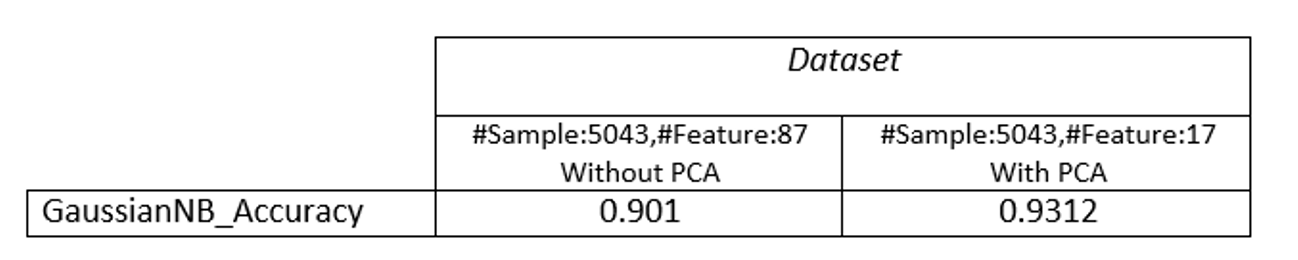
\includegraphics[scale=.26]{figfoj1}
 \caption{Accuracy in two modes}
\label{fig_foj1}
\end{figure}
Figure \ref{fig_foj2} shows the efficacy of different portions of the validation data used with different folds versus correct classification rate for the GNB method. As we can see, the maximum value for CCR obtained with folds is 3.5\% for this method. 
\begin{figure}
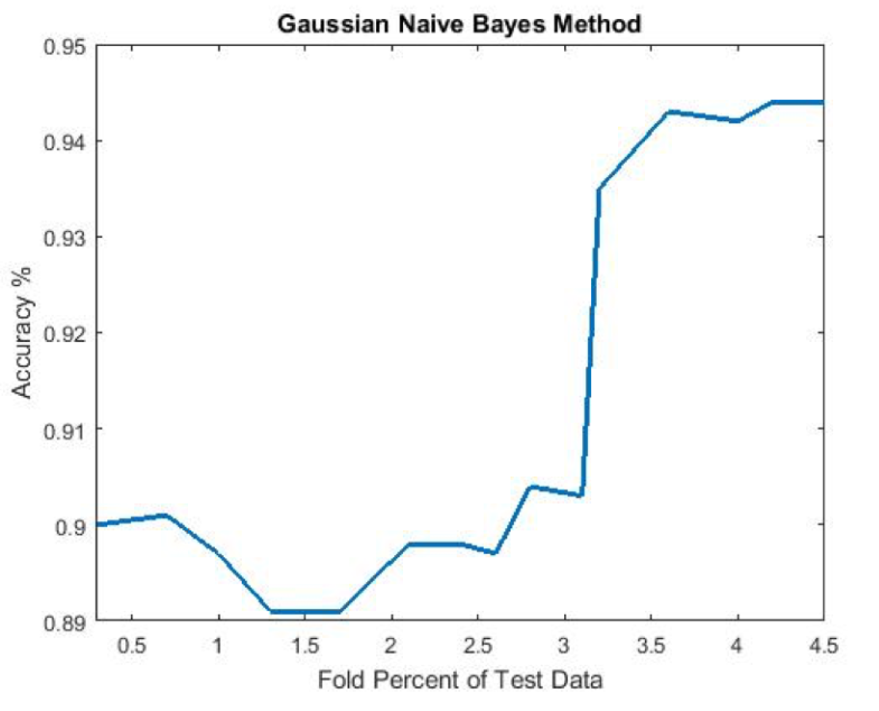
\includegraphics[scale=.38]{figfoj2}
 \caption{Accuracy with different fold percent of test data}
\label{fig_foj2}
\end{figure}

Another challenging issue is to find the best threshold for the best correlation (0.1) which is shown in figure \ref{fig_foj3}.
\begin{figure}
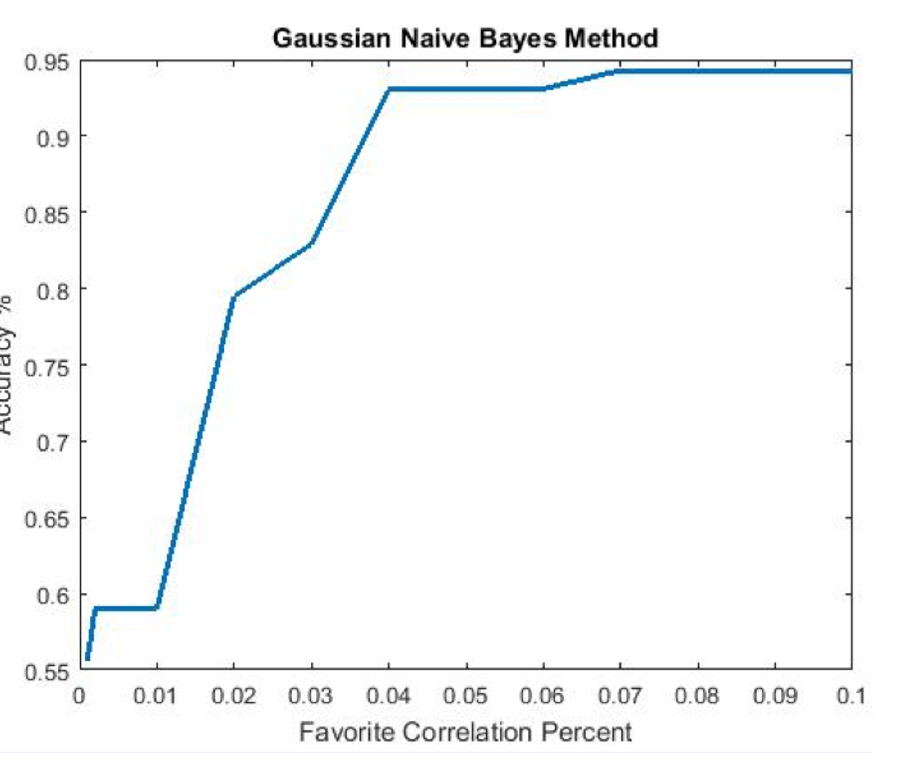
\includegraphics[scale=.38]{figfoj3}
 \caption{Accuracy with different fold percent of test data}
\label{fig_foj3}
\end{figure}
Here ( Figure \ref{fig_foj4} ) are the results of GNB classification when we did not apply PCA. As we explained before, this classifier is trying to figure out that a movie is winning the best picture or nominated for the best picture (nominee classifier). As we can see, the high precision means a low amount of false positivs which indicates if a movie will win in the future and also our classifier has proved this fact.

\begin{figure}
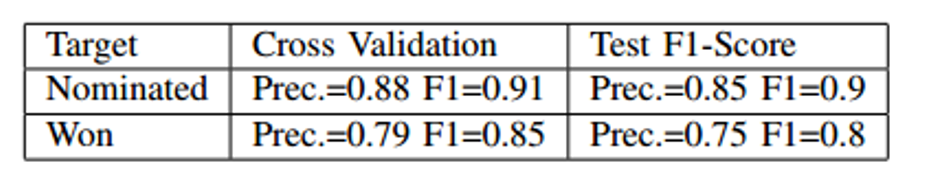
\includegraphics[scale=.35]{foj4}
 \caption{Evaluation of GNB }
\label{fig_foj4}
\end{figure}

In the following, we applied Forward Selection(FS) and Backward Elimination(BE) in order to find the best features. We provided two different scripts in python which simulate FS and BE method. After applying these methods, we found the number of best features as the following in the figure \ref{fig_foj5}.

\begin{figure}
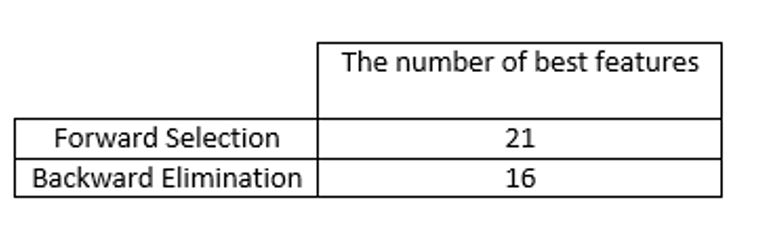
\includegraphics[scale=.35]{foj5}
 \caption{Evaluation of GNB in terms of best features}
\label{fig_foj5}
\end{figure}

\begin{figure}
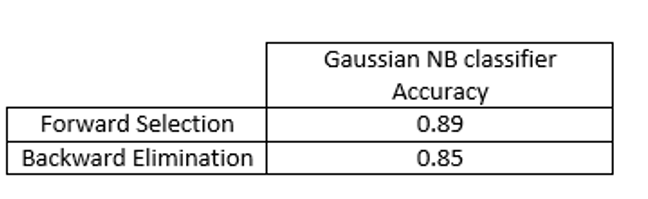
\includegraphics[scale=.4]{foj6}
 \caption{Evaluation of GNB with PCA}
\label{fig_foj6}
\end{figure}
By knowing these facts, we can evaluate the GNB classifier with these selected features as the above. As you see, FS method returned 21 features which supposed to obtain the best CCR among GNB and GNB+PCA. By feeding FS's features and BE's features to the GNB classifier, we got the results as shown in figure \ref{fig_foj6}.

It is obvious that in terms of accuracy, PCA works better than FS and BE in this context. GNB is evaluated with the forward selection method in figure \ref{fig_foj7}.

\begin{figure}
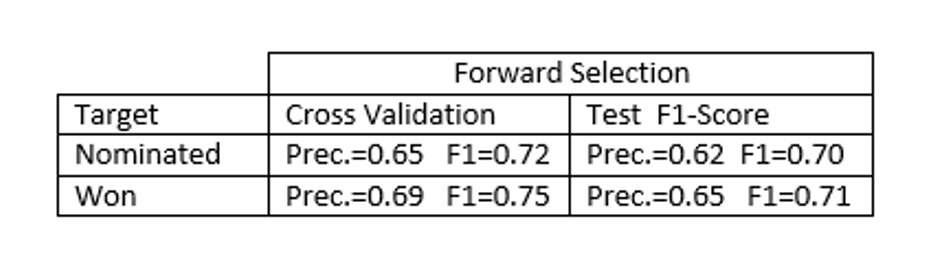
\includegraphics[scale=.35]{foj7}
 \caption{Evaluation of GNB with FS}
\label{fig_foj7}
\end{figure}
GNB evaluation with Backward Elimination method in the Figure \ref{fig_foj8}.


\begin{figure}
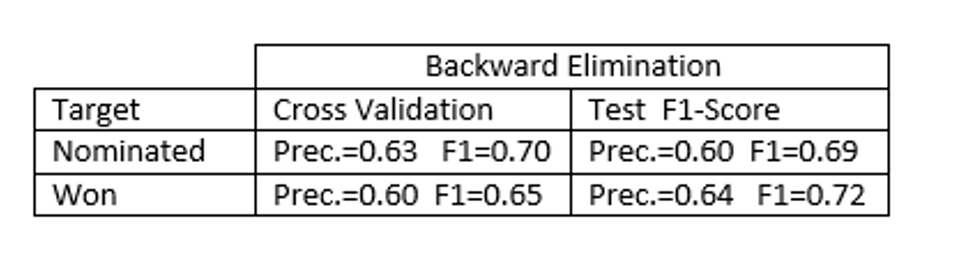
\includegraphics[scale=.35]{foj8}
 \caption{Evaluation of GNB with BE}
\label{fig_foj8}
\end{figure}

	\subsubsection{AdaBoost}
			\label{adaboost}
			Adaptive boosting is also one of the best learners that we have tried. What basically this classifier/regressor does is that it takes advantage of a number of weak learners to create a strong learner. As mentioned in \cite{adaboost}, unlike support vector machines and neural nets, the training phase of AdaBoost only selects features which have predictive power; hence, faster running time even when a lot of features are around. But what we were surprised about was the fact that unlike SVMs we did not spend a significant amount of time and trial/error to tune the classifier. In fact, in our very first attempt we got results that were clearly better than those of the SVMs. (We will elaborate on the results later). For regression/classification we used the following setting:\\
AdaBoostRegressor(DecisionTreeRegressor(max\_depth=20),\\
n\_estimators=300,random\_state=None)\\
AdaBoostClassifier(DecisionTreeClassifier(max\_depth=1),\\
algorithm="SAMME",n\_estimators=200)

In fact, the base estimator that is used here is a Decision Tree. Moreover, we are using the discrete version of the AdaBoost (SAMME) as we are interested in getting class labels as predictions rather than class probabilities.
			
			\subsubsection{Perceptrons}
			Another approach we tried was Perceptrons. Ideally, perceptrons would be able to separate the data linearly \cite{perceptron}, into nominees and non-nominees, and then winners and losers. After performing 10-fold cross-validation on our training set, we were able to tune the parameters to the following:
			\begin{itemize}
				\item For nominations, the classifier was regularized using \emph{l2} with the default value of 0.0001 in order to emphasize the more significant features.
				\item For wins, the classifier was regularized using \emph{l1} with a much smaller value 0.00001 than the default.
			\end{itemize}
			These two settings showed the most promising results during cross-validation.
			These were the best tuning parameters possible given the data's non-linear distribution.
			
			\subsubsection{Neural Networks (MLPs)}
			The last approach in this section was neural nets \cite{anns} (or multi-layered perceptrons) as they are called in \emph{scikit-learn} \cite{skl-anns}. These were also run through cross-validation (10-fold), and tuned for the best possible performance.
			\begin{itemize}
				\item Net Structure:
				\begin{itemize}
					\item For nominations, the network consists of 1 hidden layer of 200 nodes. This yielded the best results during cross-validation.
					\item For wins, the network size was increased to accommodate two hidden layers of 200 and 250 nodes respectively.
				\end{itemize}
				\item Activation Function:
					\newline
					The most effective activation function after cross-validation was found to be the default function \emph{relu} for both nominations and wins.
				\item Solver:
					\begin{itemize}
						\item For nominations, the most effective solver was found to be the stochastic gradient descent solver \emph{sgd}.
						\item For wins, the most effective solver was found to be the default solver \emph{adam}.
					\end{itemize}
				\item Regularization:
					\begin{itemize}
						\item For nominations, by keeping the regularization term \emph{alpha} at the default, we obtained the best average F1-score.
						\item For wins, we obtained the best results by increasing the value of the regularization term from its default 0.0001 to 0.001.
					\end{itemize}
			\end{itemize}
			
		\subsection{Regression}\label{subsec:regression}
			In this section, and as a further attempt to check the suitability of the data for the task at hand, we added regression in order to predict the total number of awards a movie would win. The regressors used in this experiment are:
			\begin{itemize}
				\item Linear Regression
				\item SVM Regressors
				\item AdaBoost Regressors
			\end{itemize}
			These are discussed in detail below.
			
			\subsubsection{Support Vector Regressors (SVRs)}
			Covered in \ref{svm}.
			
			\subsubsection{AdaBoost}
			Covered in \ref{adaboost}.			
			
			\subsubsection{Linear Regression}
			For linear regression, and after experimenting with all possible variations of the tuning parameters, the best possible fit was with its default settings, i.e. $fit\_intercept=True$, and $normalize=False$. The $normalize$ setting was set to $False$ mainly due to the fact that the dataset was already scaled earlier in the data preprocessing step. Linear regression, much like the perceptron, would try to estimate a line that runs closest to as much as possible of the points in the set, and use the equation from that estimated line in order to predict the dependent variable (in this case, the number of awards).
	
	\section{Results}
		This section contains the results of testing our classifiers on the test set that was generated using the techniques discussed in section \ref{train_test_set}.
		All classifiers were tested on the test-set and evaluated based on their precision, recall, and F1-scores. All regressors were also evaluated using the same test set, and evaluated based on their $R^2$ score.		
		\begin{figure}
			\centering
			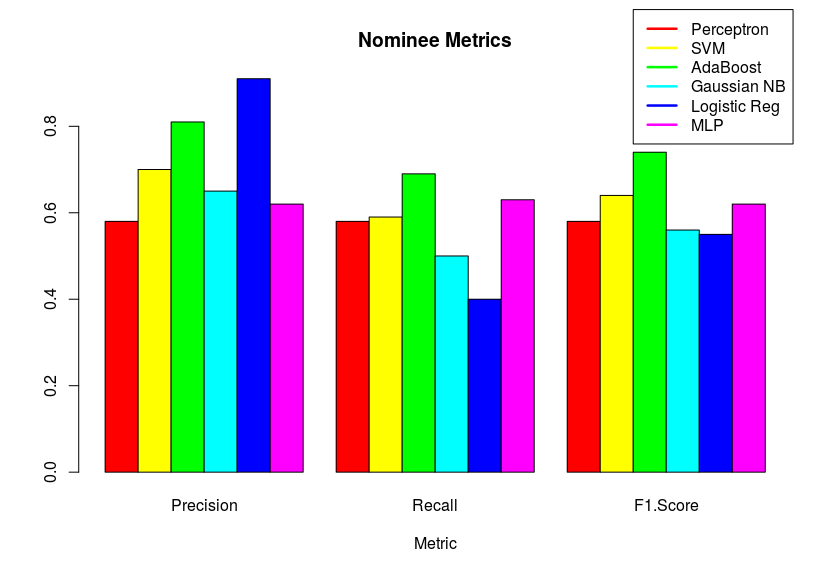
\includegraphics[scale=0.4]{metrics_nom}
			\caption{Nomination Classifier Results}
			\label{fig_metrics_nom}
		\end{figure}
		\begin{figure}
			\centering
			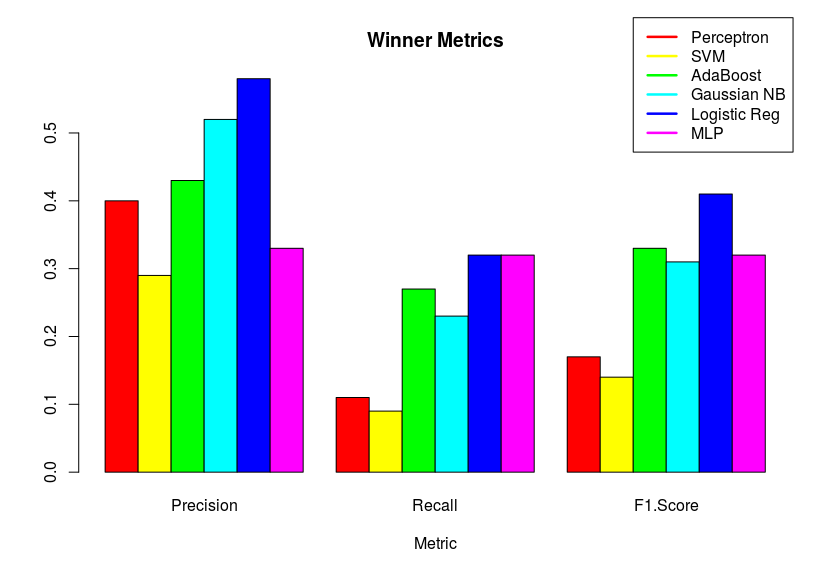
\includegraphics[scale=0.4]{metrics_win}
			\caption{Results for win classifiers}
			\label{fig_metrics_win}
		\end{figure}	
		\begin{table}
			\centering
			\begin{tabular}{|c|c|c|c|}
				\hline
				Algorithm & Precision & Recall & F1-score \\
				\hline
				Perceptron & 0.58 & 0.58 & 0.58 \\
				SVM & 0.70 & 0.59 & 0.64 \\
				AdaBoost & 0.81 & 0.69 & 0.74 \\
				Gaussian NB & 0.65 & 0.50 & 0.56 \\
				Logistic Regression & 0.91 & 0.40 & 0.55 \\
				MLPs & 0.62 & 0.63 & 0.62 \\
				\hline
			\end{tabular}
			\caption{Nomination Classifier Results}
			\label{tab:nom_metrics}
		\end{table}
		\begin{table}
			\centering
			\begin{tabular}{|c|c|c|c|}
				\hline
				Algorithm & Precision & Recall & F1-score \\
				\hline
				Perceptron & 0.40 & 0.11 & 0.17 \\
				SVM & 0.29 & 0.09 & 0.14 \\
				AdaBoost & 0.43 & 0.27 & 0.33 \\
				Gaussian NB & 0.52 & 0.23 & 0.31 \\
				Logistic Regression & 0.58 & 0.32 & 0.41 \\
				MLPs & 0.33 & 0.32 & 0.32 \\
				\hline
			\end{tabular}
			\caption{Wins Classifier Results}
			\label{tab:win_metrics}
		\end{table}		
		\subsection{Classifiers}
		The results for the best picture award nominations can be seen in figure \ref{fig_metrics_nom}, whereas those for winners can be found in figure \ref{fig_metrics_win}.
		\newline
		\textbf{Nominations:} As can be seen in figure \ref{fig_metrics_nom}, the best precision was achieved with the logisitc regressor, followed closely by AdaBoost. The best recall was achieved by AdaBoost, and then MLPs. Not surprisingly, the best F1 measure was achieved by AdaBoost, and in second place was the SVM. The detailed results are given in table \ref{tab:nom_metrics}.
		\newline
		\textbf{Wins:} As can be seen in figure \ref{fig_metrics_win}, the best precision was achieved with -again- the logistic regressor, followed closely by the gaussian naive bayes classifier. The best recall was a tie between the logistic regressor and MLPs. But, eventually, the best F1-score was achieved by the logistic regressor, similar to the work done in \cite{ref4}. The detailed results are given in table \ref{tab:win_metrics}.		
		\subsection{Regressors}
		As was discussed in section \ref{subsec:regression}, the regressors were used in order to estimate the total number of awards a movie would win. According to our tests, the best performance was achieved using AdaBoost, then at a close second was the SVM regressor, and finally at a very distant third, the linear regressor. The details can be seen in table \ref{tab:awd_r2}.
		\begin{table}
			\centering
			\begin{tabular}{|c|c|}
				\hline
				Regressor & $R^2$ Score \\
				\hline
				AdaBoost & 0.60 \\
				SVM Regressor & 0.40 \\
				Linear Regression & $-4.13760627174991E+29$ \\
				\hline
			\end{tabular}
			\caption{Number of Awards Regression Results}
			\label{tab:awd_r2}
		\end{table}	
	\section{Discussion and Future Work}
		As can be seen from the previous section, our classifiers performed adequately when it came to predicting whether a movie would be nominated or not. With a maximum F1 score (AdaBoost) of 0.74, we can say that the classifier is certainly not being overfit, and is giving reasonable predictions. It should also be noted that AdaBoost did in some part rely on decision trees, which are better suited to model cognitive decision making as opposed to the numerical estimations the other classifiers make. It is also worth noting that decision trees are also better suited to dealing with the categorical nature of our dataset.
		\par
		We deduce that the reason our linear separators did not work so well is due to two major issues:
		\begin{enumerate}
			\item The data is not linearly separable, as is evident by the performance of the perceptrons and linear regressor.
			\item The data is severely unbalanced. For each year there is a huge amount of movies, only a small portion of which gets nominated, and only one of those wins per year.
		\end{enumerate}
		Another lingering issue is that we had to augment our dataset with data about nominations and a movie's IMDB score in order to get reasonable performance. That implies that, on its own, movie popularity measured by its social media likes (as well as those of its creators, actors, ...etc.) is not enough to adequately predict if a movie is going to get nominated or not. It certainly is not enough to predict if a movie would win or not, as is evident by the low metrics recorded for that scenario (even after including data about nominations).
		\par
		One other avenue we explored was whether or not a movie's nomination or win could be influenced by its budget, as it would typically include its advertising budget as well. This was rapidly disproved during the feature selection stage, where the correlation between the movie's budget and nomination/win was statistically insignificant; i.e. between 0.1 and -0.1 as measured by pearson's correlation coefficient.
		\par
		Given more time, we would like to explore other classification alternatives, for instance decision trees and random forests. We would also like to augment the dataset with user and critic reviews as those can be a strong indicator of how well a movie is performing with respect to the general public. This would initially involve sentiment analysis and other techniques to get a better sense of how a movie is received by other online presence.
		\par
		Another approach would be to try clustering, and see if we can group movies based on how similar they are, which might be able to indicate winning groups. This is as opposed to trying to classify  and separate them.
	
\section{Contributions of Project Members}
\subsection{Fojan Babaali}
Fojan was responsible for implementing and experimenting with the gaussian naive bayes classifier. She collaborated with Maryam in exploring related work in literature. Moreover, she contributed in preparing the mid-term/final reports and the final presentation.

\subsection{Maryam Honari Jahromi}
Maryam was responsible for implementing the logistic regression classifier. She collaborated with Fojan in exploring related work. She also collaborated with Ali in refining the dataset and repeating the work of Chuan Sun (creator of the dataset). Moreover, she contributed in preparing the mid-term/final reports and the final presentation.

\subsection{Omar Elazhary}
Omar was in charge of the perceptrons, linear regression and neural networks. He also handled data preprocessing and feature correlation results. He, as well, contributed in preparing the mid-term/final reports. Furthermore, he contributed in preparing result visualizations and presenting in class.

\subsection{Ali Mashreghi}
Ali was in charge of the SVMs and AdaBoost. He collaborated with Maryam in refining the dataset, repeating the work of Chuan Sun. He also collected historical data. He, as well, contributed in preparing the mid-term/final reports. Furthermore, he contributed in preparing and presenting the presentation.	
	
	\begin{thebibliography}{1}

 \bibitem{ref6} \url{http://www.economist.com/blogs/economist-explains/2015/01/economist-explains-14}, Accessed on 10/02/16
\bibitem{ref7} \url{https://www.kaggle.com/datasets?sortBy=hottest&group=featured&search=imdb}, Accessed on 10/02/16
\bibitem{ref8} \url{https://www.youtube.com/watch?v=qhfxo8xPNGU}, Accessed on 10/03/16
\bibitem{ref1}  \url{http://insights.principa.co.za/data-scientists-predict-oscar-winners} (February 2016)
\bibitem{ref2} Krauss, Jonas, Stefan Nann, Daniel Simon, Peter A. Gloor, and Kai Fischbach.``Predicting Movie Success and Academy Awards through Sentiment and Social Network Analysis." In ECIS, pp. 2026-2037. 2008.
\bibitem{ref3}  \url{http://maxmelnick.com/2016/05/18/predicting-oscar-nominations.html} (May 2016)
\bibitem{ref4} Barber, Stephen, Kasey Le, and Sean O’Donnell.``Predicting the 85th Academy Awards." (2012).
\bibitem{ref5} \url{https://blog.nycdatascience.com/student-works/machine-learning/movie-rating-prediction/}, Accessed on 10/03/16
\bibitem{ref6} \url{http://scikit-learn.org/stable/modules/svm.html}
\bibitem{refFoj} \url{Kessy, Agnan, Alex Lewin, and Korbinian Strimmer. "Optimal whitening and decorrelation." arXiv preprint arXiv:1512.00809 (2015).}
\bibitem{refCreator} \url{https://blog.nycdatascience.com/student-works/machine-learning/movie-rating-prediction/}
\bibitem{adaboost} \url{https://en.wikipedia.org/wiki/AdaBoost}
\bibitem{perceptron} Han, J., Pei, J. and Kamber, M., 2011. \emph{Data mining: concepts and techniques}. Elsevier.
\bibitem{anns} \url{https://en.wikipedia.org/wiki/Artificial_neural_network} accessed on 12/01/2016
\bibitem{skl-anns} \url{http://scikit-learn.org/stable/modules/generated/sklearn.neural_network.MLPClassifier.html} accessed on 12/01/2016

\bibitem{maryamref20} Kaplan, ``And the Oscar Goes to… A Logistic Regression Model for Predicting Academy Award Results" In Jaep25 ,2006
\end{thebibliography}
	
\end{document}